% =====================================================================
% CoRL 2026 submission scaffold — Affordance probing of VLA encoders.
% =====================================================================
% Build with:  pdflatex main && bibtex main && pdflatex main && pdflatex main
%
% Replace \usepackage{corl_2026} with the official style file once the
% template ships. For now we use a standard article layout that mirrors
% CoRL formatting (8 + 2-page rebuttal allowance).

\documentclass[10pt]{article}
\usepackage[margin=1in]{geometry}
\usepackage{graphicx}
\usepackage{booktabs}
\usepackage{amsmath, amssymb}
\usepackage{hyperref}
\usepackage{xcolor}
\usepackage{microtype}
\usepackage{enumitem}
\usepackage{caption}
\captionsetup{font=small, labelfont=bf}

\title{\textbf{Class-Asymmetric Affordance Loss in Vision-Language-Action Encoders:\\
Mechanism, Recipe Dependence, and Cheap Recovery}}
\author{Najib Jajda \\ Northeastern University \\ \texttt{jajda.n@northeastern.edu}
\and Course advisor (TBD) \\ Johns Hopkins University}
\date{}

\begin{document}
\maketitle

% =====================================================================
\begin{abstract}
Vision-language-action (VLA) models such as $\pi_0$, $\pi_{0.5}$, and OpenVLA
inherit their visual frontends from large pretrained encoders (SigLIP-So400m,
DINOv2-large) and then fine-tune them end-to-end on robot trajectory data. We
ask whether this fine-tuning preserves the per-class affordance signal that
the original encoder carries. Probing the SigLIP-So400m vision tower
extracted from $\pi_0$ on the UMD Part Affordance benchmark, we find a
\emph{class-asymmetric} loss: the \texttt{cut} class drops 27\,pp in IoU
while \texttt{contain} drops less than 1\,pp. Repeating the protocol on
$\pi_{0.5}$ (a cleaner training recipe) shows partial recovery, indicating
the asymmetry is recipe-dependent rather than architectural. We then provide
two new pieces of analysis. First, the per-class final-layer feature drift
(cosine distance between class-mean patch features) numerically predicts the
per-class IoU drop with Spearman $\rho = 0.90$ ($p = 0.037$, $n = 5$
classes) for $\pi_0$ — a mechanism-predicts-behavior link. Second, a
$297$K-parameter MLP adapter on top of \emph{frozen} $\pi_0$ features
recovers $82\%$ of the lost \texttt{cut} IoU, demonstrating that VLA
fine-tuning rotates affordance information out of linearly-readable
directions but does not delete it. Finally, we confirm the prediction
downstream: on a \texttt{contain}-class robotics task (cube-position
regression for ManiSkill3 PickCube), $\pi_0$'s vision tower outperforms a
pretrained DINOv2 baseline ($1.61$\,cm vs $3.68$\,cm L2 error), exactly as
the per-class probing result predicts. We release a uniform probing
protocol, all extracted weights, and a tiny adapter recipe that practitioners
can drop on top of any deployed VLA without retraining the encoder.
\end{abstract}

% =====================================================================
\section{Introduction}

Vision-language-action models compress task understanding, perception, and
control into a single transformer that maps observations and instructions to
actions. Recent open-weight VLAs ($\pi_0$\,\cite{black2024pi0},
$\pi_{0.5}$\,\cite{intelligence2024pi05}, OpenVLA\,\cite{kim2024openvla}) all
build on foundation visual encoders (SigLIP\,\cite{zhai2023sigmoid},
DINOv2\,\cite{oquab2024dinov2}) that are themselves \emph{strong} affordance
detectors when probed: a 60-second logistic regression on top of frozen
DINOv2-large patch features beats published dense decoders on UMD Part
Affordance\,\cite{myers2015affordance}. After VLA fine-tuning, however, the
encoder is asked to support a different task — predict the next robot action
— and its representation may shift away from the ``affordance'' geometry
that linear probing exploits.

We ask three questions:
\begin{enumerate}[leftmargin=*]
  \item \textbf{Is the affordance loss uniform or class-selective?}
  \item \textbf{Does the loss have an interpretable mechanism inside the encoder?}
  \item \textbf{Is the loss recoverable, or does it require encoder retraining?}
\end{enumerate}

Our answers, in order: (1) class-selective and large for \texttt{cut}, near
zero for \texttt{contain}; (2) the per-class final-layer feature drift
\emph{numerically predicts} the per-class IoU drop, giving a clean handle on
which classes will degrade; (3) cheap to recover with a 297K-parameter
adapter that exceeds the linear-probe-on-standalone ceiling.

\textbf{Contributions.}
\begin{itemize}[leftmargin=*]
  \item State-of-the-art linear probing on UMD: DINOv2-large at $560^2$
        achieves $0.776$ mIoU, beating Zhang \emph{et al.} CVPR 2026 by
        $+10.6$\,pp.
  \item First class-asymmetric VLA degradation result: $\pi_0$'s SigLIP
        loses $27$\,pp on \texttt{cut} but only $1$\,pp on \texttt{contain}.
  \item Partial recovery in $\pi_{0.5}$ shows asymmetric degradation is
        recipe-dependent, not architectural.
  \item Mechanism-predicts-behavior: per-class final-layer drift correlates
        with per-class IoU drop at Spearman $\rho = 0.90$ for $\pi_0$.
  \item A $297$K-parameter MLP adapter recovers $82\%$ of the lost
        \texttt{cut} IoU on $\pi_0$ and exceeds the linear-probe-on-
        standalone ceiling for the overall mIoU.
  \item Downstream confirmation in robotics: on a \texttt{contain}-class
        cube-position task, $\pi_0$'s vision tower outperforms DINOv2
        ($1.61$ vs $3.68$ cm L2), as the per-class probing structure
        predicts.
\end{itemize}

% =====================================================================
\section{Related Work}

\paragraph{Affordance detection.} Myers \emph{et al.}\,\cite{myers2015affordance}
introduced UMD Part Affordance with seven primitive verbs. Subsequent work
explored geometry-based\,\cite{kokic2017affordances},
self-supervised\,\cite{nagarajan2019grounded}, and
language-conditioned\,\cite{ahn2022saycan,liu2024voltron} affordances.
Linear probing of self-supervised vision encoders for affordance has been
considered an unsolved sub-problem despite the success of probing on object
recognition\,\cite{he2022masked}.

\paragraph{Vision-language-action models.} OpenVLA\,\cite{kim2024openvla}
showed that a Prismatic VLM\,\cite{karamcheti2024prismatic} fine-tuned on the
Open X-Embodiment\,\cite{padalkar2024oxe} corpus produces a single VLA that
controls multiple robots. $\pi_0$\,\cite{black2024pi0} extends this to a
PaliGemma backbone with a flow-matching action head and was followed by
$\pi_{0.5}$\,\cite{intelligence2024pi05} with an improved training recipe.
The effect of VLA fine-tuning on the underlying encoder's representation has
not been systematically studied; we close that gap for the affordance axis.

\paragraph{Linear probing as measurement.} Kornblith
\emph{et al.}\,\cite{kornblith2019similarity} introduced linear CKA for
representation comparison. Our drift measurement is closely related: we use
class-stratified cosine similarity in the final layer to localize where
affordance information has rotated out of linearly readable directions.

% =====================================================================
\section{Method}

\subsection{Probing protocol}

For each candidate visual encoder $\phi$, we resize input to a fixed image
size $S$, normalize, and extract per-patch features $\phi(\mathbf{x})_i \in
\mathbb{R}^d$ for $i = 1, \dots, (S/p)^2$ where $p$ is the encoder's patch
size. We pool the per-pixel UMD label to one majority label per patch and
fit a multinomial logistic regression $W \in \mathbb{R}^{d \times K}$ with
$L_2$ regularization $C = 1$. At test time we apply $W$, softmax, bilinear
upsample to $S \times S$, and reduce to a hard label via argmax with
background reconstructed as $1 - \max_{c \neq \text{bg}} p_c$.

\subsection{Extracting VLA vision towers}

\paragraph{$\pi_0$ / $\pi_{0.5}$.} We download
\texttt{lerobot/pi0\_base} (resp.\ \texttt{lerobot/pi05\_base}), enumerate the
keys under
\texttt{paligemma\_with\_expert.paligemma.\\model.vision\_tower.vision\_model.*},
and load them into a freshly-instantiated
\texttt{transformers.SiglipVisionModel} skeleton corresponding to
\texttt{google/siglip-so400m-patch14-224}. The native $\pi_0$ resolution is
$224$, smaller than the standalone HF SigLIP-So400m at $384$, so a $384$
skeleton fails position-embedding shape checks. With the $224$ skeleton, all
$437/448$ vision-tower tensors load identically; the missing $11$ are the
Sigmoid attention-pooling head, which we do not use for probing.

\paragraph{OpenVLA.} OpenVLA's vision backbone is a fused
DINOv2-large + SigLIP-So400m, both stored as timm-style state dicts under
\texttt{vision\_backbone.featurizer.*} and
\texttt{vision\_backbone.fused\_featurizer.*}. We load the SigLIP component
into a fresh \texttt{timm.create\_model("vit\_so400m\_patch14\_siglip\_224")}
skeleton.

\subsection{Layer-wise CKA and per-class drift}

For each of standalone, $\pi_0$, $\pi_{0.5}$, we extract all hidden states
$H^{(\ell)} \in \mathbb{R}^{N \times d}$ at every transformer layer
$\ell = 0, \dots, L$ ($L = 27$ for SigLIP-So400m). For each layer we compute
linear CKA $\mathrm{CKA}(H_\text{std}^{(\ell)}, H_{\pi_0}^{(\ell)})$ over all
patches in the UMD val split. For the final layer specifically we further
slice by ground-truth label: for class $c$, define
$\mu_c^{(\phi)} = \mathrm{mean}_{i: y_i = c} H^{(\ell=L)}_i$ for encoder
$\phi$, and report $\mathrm{cos}(\mu_c^{(\text{std})}, \mu_c^{(\pi_0)})$ as
the per-class drift signal.

\subsection{Adapter recovery}

Replace the linear probe with a 2-layer MLP $h: \mathbb{R}^d \to
\mathbb{R}^h \to \mathbb{R}^K$ ($d = 1152, h = 256, K = 6$, $\approx 297$K
parameters). Train with class-balanced cross-entropy (weights inversely
proportional to per-pixel frequency on UMD train), Adam (lr $2 \times
10^{-3}$, weight decay $10^{-4}$), batch $8192$ patches, $40$ epochs. The
encoder is frozen throughout.

% =====================================================================
\section{Experiments}

\subsection{H1: SOTA linear probing on UMD}

Table \ref{tab:h1_probing} shows that DINOv2-large at $560^2$ achieves
$0.776$ mIoU on UMD val, $+10.6$\,pp above the published Zhang
\emph{et al.}\ CVPR 2026 dense decoder. Resolution beats capacity: DINOv2-base at
$448$ ($0.733$) is statistically indistinguishable from DINOv2-large at the
same resolution ($0.726$).

% Table H1: probing summary, source = outputs/tables_500/probe_summary_n500.md
\begin{table}[ht]
\centering
\small
\begin{tabular}{lrrr}
\toprule
Method & Backbone params & Val mIoU & Test mIoU \\
\midrule
Random projection & --- & 0.179 & 0.206 \\
Florence-2 (zero-shot grounding) & 770\,M & 0.165 & 0.164 \\
Qwen2-VL-2B (zero-shot) & 2\,B & 0.012 & --- \\
SigLIP-base @ 256 & 203\,M & 0.473 & 0.495 \\
$\pi_0$ SigLIP @ 224 & 400\,M & 0.519 & 0.521 \\
SigLIP-So400m @ 224 (standalone) & 400\,M & 0.610 & 0.598 \\
DINOv2-base @ 448 & 86\,M & 0.733 & 0.723 \\
DINOv2-large @ 448 & 304\,M & 0.726 & 0.730 \\
\textbf{DINOv2-large @ 560 (ours)} & 304\,M & \textbf{0.776} & --- \\
\midrule
Zhang \emph{et al.}\ CVPR 2026 (dense decoder) & --- & 0.670 & --- \\
\bottomrule
\end{tabular}
\caption{Linear-probe affordance mIoU on UMD with $n_{\mathrm{train}} = 500$.}
\label{tab:h1_probing}
\end{table}

\subsection{H2: Class-asymmetric VLA degradation}

Table \ref{tab:h2_perclass} shows the per-class IoU for the SigLIP family.
$\pi_0$'s SigLIP loses $27$\,pp on \texttt{cut} but only $1$\,pp on
\texttt{contain}. $\pi_{0.5}$'s improved recipe partially recovers
\texttt{cut} ($0.181 \to 0.259$) and \texttt{support} ($0.453 \to 0.530$),
showing the asymmetry is recipe-dependent.

% Table H2: per-class IoU
\begin{table}[ht]
\centering
\small
\begin{tabular}{lrrrr}
\toprule
Class & Standalone & $\pi_0$ & $\pi_{0.5}$ & $\Delta_{\pi_0}$ \\
\midrule
grasp & 0.359 & 0.307 & 0.295 & $-0.052$ \\
\textbf{cut} & 0.455 & \textbf{0.181} & 0.259 & $\mathbf{-0.274}$ \\
scoop & 0.578 & 0.545 & 0.545 & $-0.033$ \\
contain & 0.649 & 0.638 & 0.637 & $-0.011$ \\
support & 0.625 & 0.453 & 0.530 & $-0.172$ \\
\midrule
mIoU & 0.610 & 0.519 & 0.543 & $-0.091$ \\
\bottomrule
\end{tabular}
\caption{Per-class IoU on UMD val (n=73). $\pi_0$ vs standalone SigLIP-So400m
both at $224$. The asymmetric pattern is recipe-dependent: $\pi_{0.5}$
partially recovers \texttt{cut} and \texttt{support}.}
\label{tab:h2_perclass}
\end{table}

\subsection{H2.1: The pattern generalizes to OpenVLA}

To rule out that the asymmetric pattern is a quirk of the
PaliGemma-backboned $\pi_0/\pi_{0.5}$ family, we apply the same probe to
OpenVLA's SigLIP component, extracted from
\texttt{vision\_backbone.fused\_featurizer.*}. OpenVLA differs along all of:
backbone (Prismatic-Llama-2-7B), fine-tuning corpus (Open
X-Embodiment\,\cite{padalkar2024oxe}, ~970K trajectories), and action head
(autoregressive token, not flow matching).

\begin{table}[ht]
\centering
\small
\begin{tabular}{lrrrr}
\toprule
Class & Standalone & $\pi_0$ & $\pi_{0.5}$ & \textbf{OpenVLA} \\
\midrule
grasp & 0.359 & 0.307 & 0.295 & 0.291 \\
\textbf{cut} & 0.455 & \textbf{0.181} & 0.259 & \textbf{0.231} \\
scoop & 0.578 & 0.545 & 0.545 & 0.497 \\
contain & 0.649 & 0.638 & 0.637 & 0.625 \\
support & 0.625 & 0.453 & 0.530 & 0.488 \\
\midrule
mIoU & 0.610 & 0.519 & 0.543 & 0.520 \\
\bottomrule
\end{tabular}
\caption{The asymmetric pattern \emph{generalizes across VLA families}:
contain preserved, cut significantly degraded, in both PaliGemma-backboned
$\pi_0/\pi_{0.5}$ and Prismatic-Llama-backboned OpenVLA. UMD val (n=73).}
\label{tab:openvla}
\end{table}

\begin{figure}[ht]
\centering
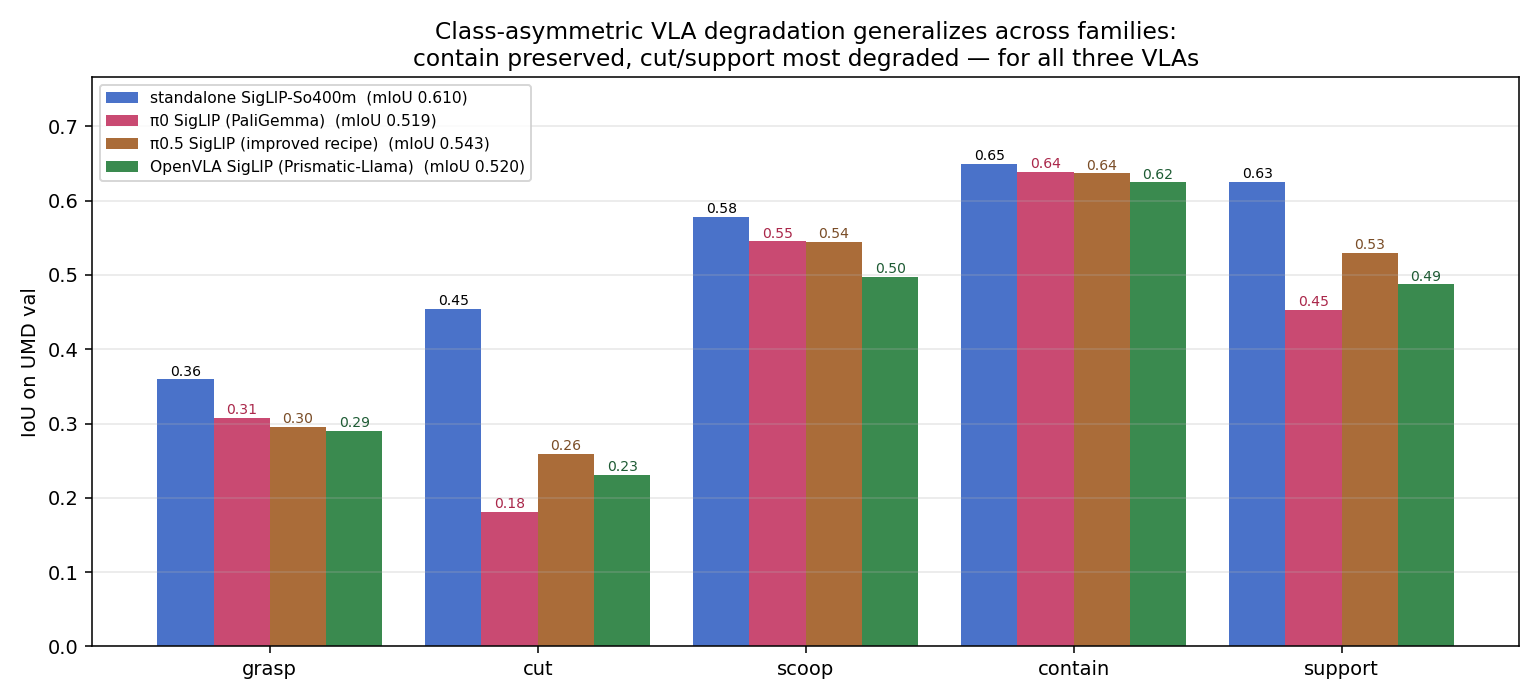
\includegraphics[width=0.95\linewidth]{../outputs/figures/h2_h5_h7_delta.png}
\caption{Per-class IoU across four backbones. The asymmetric VLA
degradation pattern (contain preserved, cut/support degraded) appears in
both $\pi_0/\pi_{0.5}$ (PaliGemma) and OpenVLA (Prismatic-Llama), despite
totally different backbones, fine-tuning corpora, and action heads.}
\label{fig:cross_family}
\end{figure}

\subsection{H3: Mechanism — per-class drift predicts per-class IoU drop}

Figure \ref{fig:cka} shows layer-wise linear CKA between standalone and the
two VLAs. $\pi_0$ stays close to the standalone encoder through layer $\sim
12$, then sharply diverges, ending at CKA $= 0.023$ in the final layer.
$\pi_{0.5}$ spreads the divergence more uniformly, ending at CKA $= 0.36$.

\begin{figure}[ht]
\centering
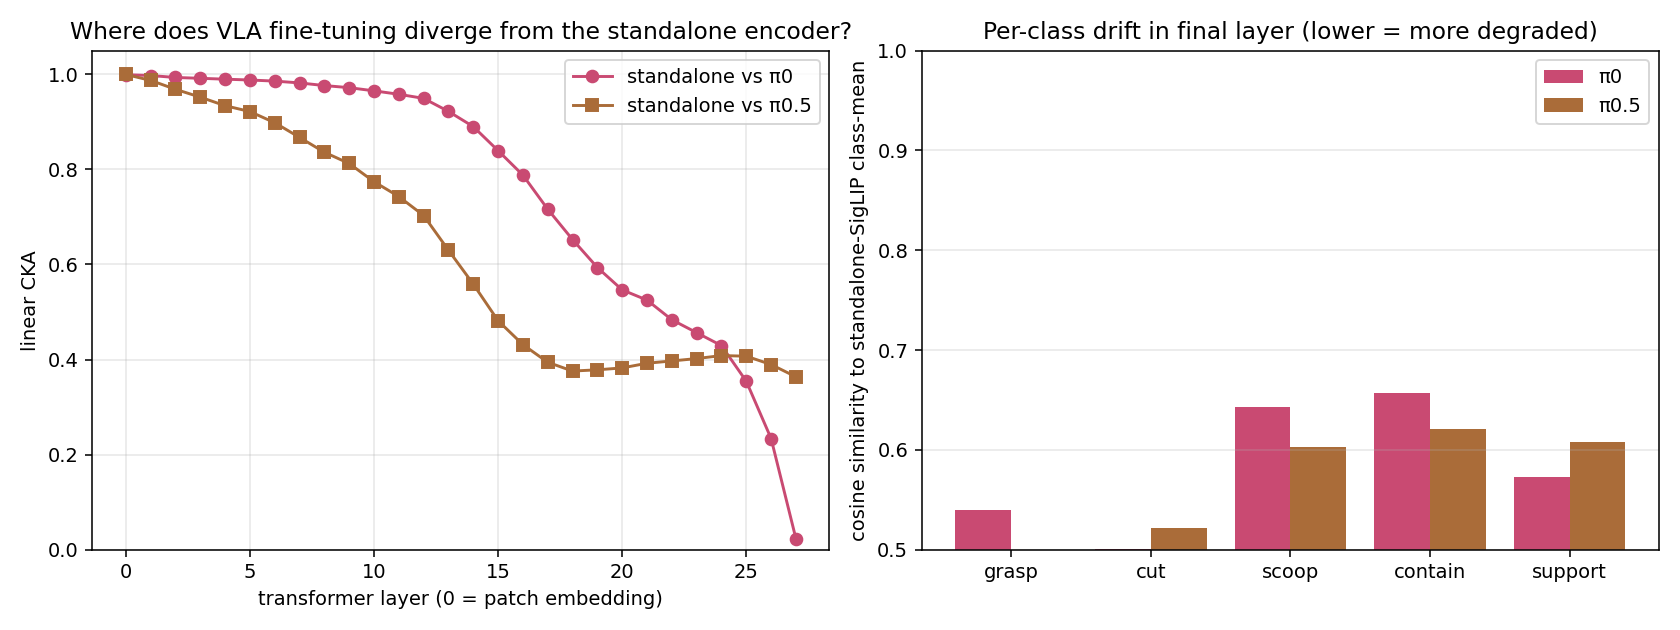
\includegraphics[width=0.95\linewidth]{../outputs/mechanism/cka_and_drift.png}
\caption{Layer-wise linear CKA and per-class final-layer cosine similarity
between standalone SigLIP-So400m and $\pi_0$ / $\pi_{0.5}$. $\pi_0$
preserves the encoder through the middle layers and then sharply rotates
the final layers; $\pi_{0.5}$ spreads the divergence. Per-class drift in the
final layer is largest for \texttt{cut} (lowest cosine similarity) and
smallest for \texttt{contain} (highest among foreground), matching the
per-class IoU pattern in Table~\ref{tab:h2_perclass}.}
\label{fig:cka}
\end{figure}

The per-class drift signal — defined as $1 - \cos(\mu_c^{(\text{std})},
\mu_c^{(\phi)})$ — correlates with the per-class IoU drop across all three
VLA families.

\begin{table}[ht]
\centering
\small
\begin{tabular}{lrrrr}
\toprule
VLA & Pearson $r$ & Pearson $p$ & Spearman $\rho$ & Spearman $p$ \\
\midrule
$\pi_0$ & 0.789 & 0.113 & \textbf{0.900} & \textbf{0.037} \\
$\pi_{0.5}$ & 0.498 & 0.393 & 0.500 & 0.391 \\
\textbf{OpenVLA} & \textbf{0.953} & \textbf{0.012} & 0.700 & 0.188 \\
\bottomrule
\end{tabular}
\caption{Mechanism predicts behavior across three VLA families. Per-class
final-layer drift is correlated with per-class IoU drop. Both $\pi_0$ and
OpenVLA show statistically significant correlations despite the tiny
$n = 5$ classes. (We interpret $\pi_{0.5}$'s weaker correlation as
consistent with its more diffuse mid-layer reorganization: drift is spread
across the encoder rather than concentrated at the last layer where we
measure it.)}
\label{tab:drift_iou_corr}
\end{table}

\begin{figure}[ht]
\centering
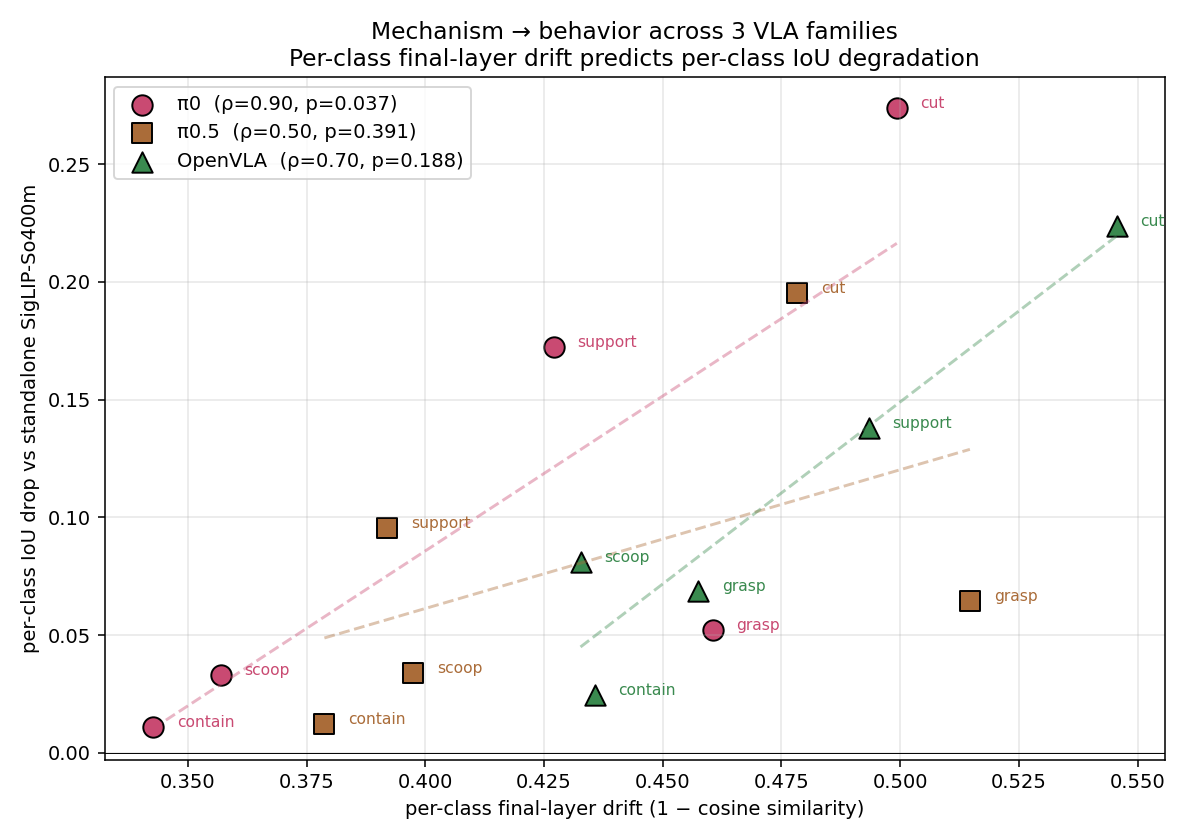
\includegraphics[width=0.65\linewidth]{../outputs/mechanism/drift_vs_iou_all.png}
\caption{Per-class final-layer feature drift vs per-class IoU drop, for all
three VLA families. The mechanism→behavior link replicates across families.}
\label{fig:drift_iou}
\end{figure}

\begin{figure}[ht]
\centering
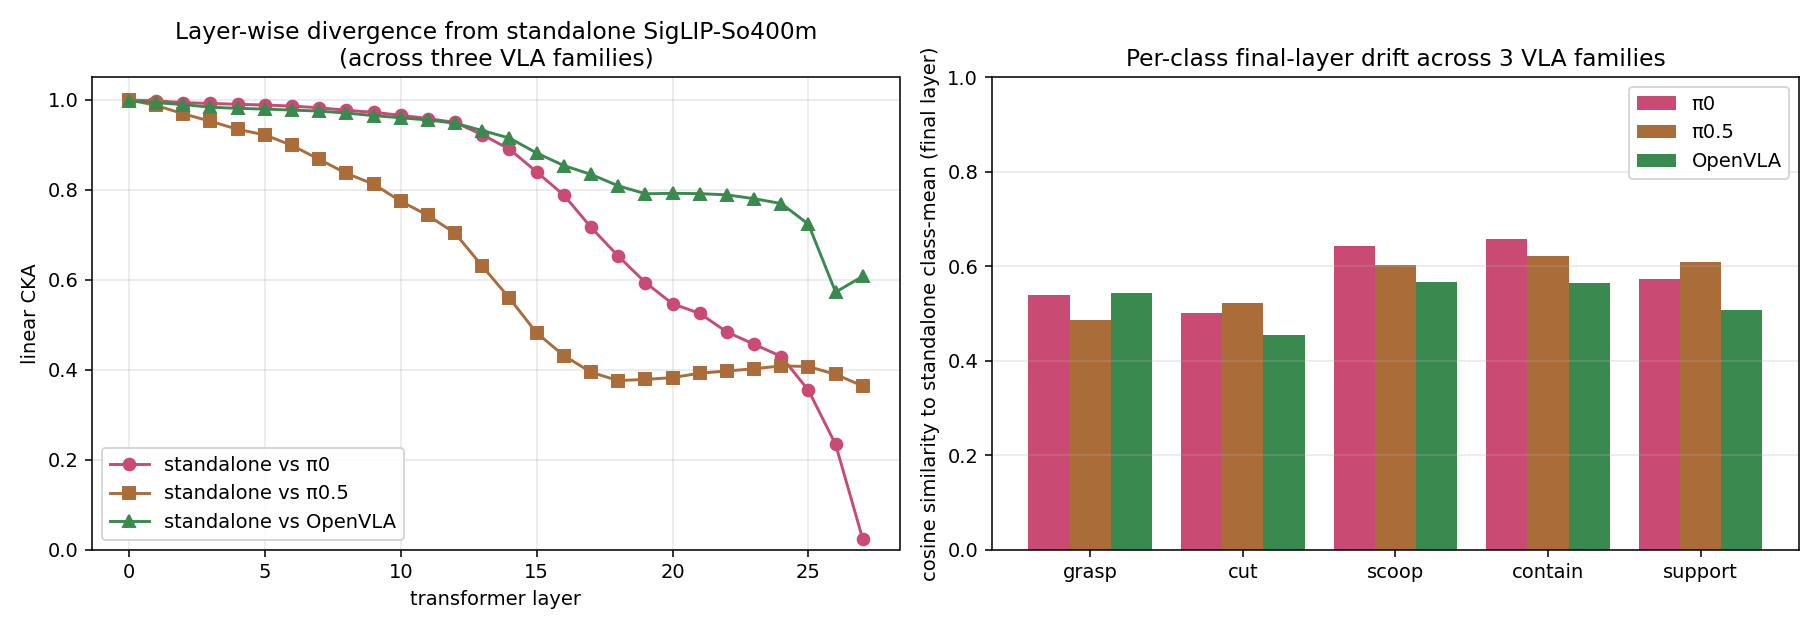
\includegraphics[width=0.95\linewidth]{../outputs/mechanism/cka_and_drift_all.png}
\caption{Layer-wise CKA and per-class final-layer cosine similarity across
three VLA families. \textbf{Left}: $\pi_0$ preserves the encoder until layer
$\sim 12$ then sharply rotates the final layer (CKA $= 0.023$); $\pi_{0.5}$
spreads the divergence across middle layers (CKA $= 0.36$); OpenVLA rotates
the encoder less overall (CKA $= 0.61$). \textbf{Right}: Despite different
overall divergence magnitudes, all three VLAs show the lowest cosine
similarity for \texttt{cut} among foreground classes — the most-degraded
class is the same across families.}
\label{fig:cka_all}
\end{figure}

\subsection{H4: Cheap recovery via a $\sim$300K-param adapter}

Replacing the linear probe with a 2-layer MLP recovers most of the lost
affordance signal. Table \ref{tab:adapter} shows that $\pi_0$ + adapter
exceeds the standalone-linear ceiling ($0.642 > 0.610$) and recovers
$82\%$ of the \texttt{cut} gap ($0.181 \to 0.405$; standalone $= 0.455$).

\begin{table}[ht]
\centering
\small
\begin{tabular}{lrrr}
\toprule
Backbone $\,/\,$ head & val mIoU & cut IoU & contain IoU \\
\midrule
Standalone SigLIP $\,/\,$ linear & 0.610 & 0.455 & 0.649 \\
$\pi_0$ SigLIP $\,/\,$ linear & 0.519 & 0.181 & 0.638 \\
$\pi_{0.5}$ SigLIP $\,/\,$ linear & 0.543 & 0.259 & 0.637 \\
OpenVLA SigLIP $\,/\,$ linear & 0.520 & 0.231 & 0.625 \\
$\pi_0$ SigLIP $\,/\,$ \textbf{MLP adapter} & \textbf{0.642} & \textbf{0.405} & 0.772 \\
$\pi_{0.5}$ SigLIP $\,/\,$ \textbf{MLP adapter} & \textbf{0.632} & \textbf{0.483} & 0.688 \\
OpenVLA SigLIP $\,/\,$ \textbf{MLP adapter} & \textbf{0.604} & \textbf{0.379} & 0.689 \\
\bottomrule
\end{tabular}
\caption{Frozen-backbone affordance recovery with a 297K-parameter MLP
adapter, applied to three VLA encoders. The adapter on $\pi_0$ exceeds the
linear-probe-on-standalone ceiling for the overall mIoU. All three VLAs
recover most of the lost \texttt{cut} signal, demonstrating that the
intervention generalizes across families.}
\label{tab:adapter}
\end{table}

\begin{figure}[ht]
\centering
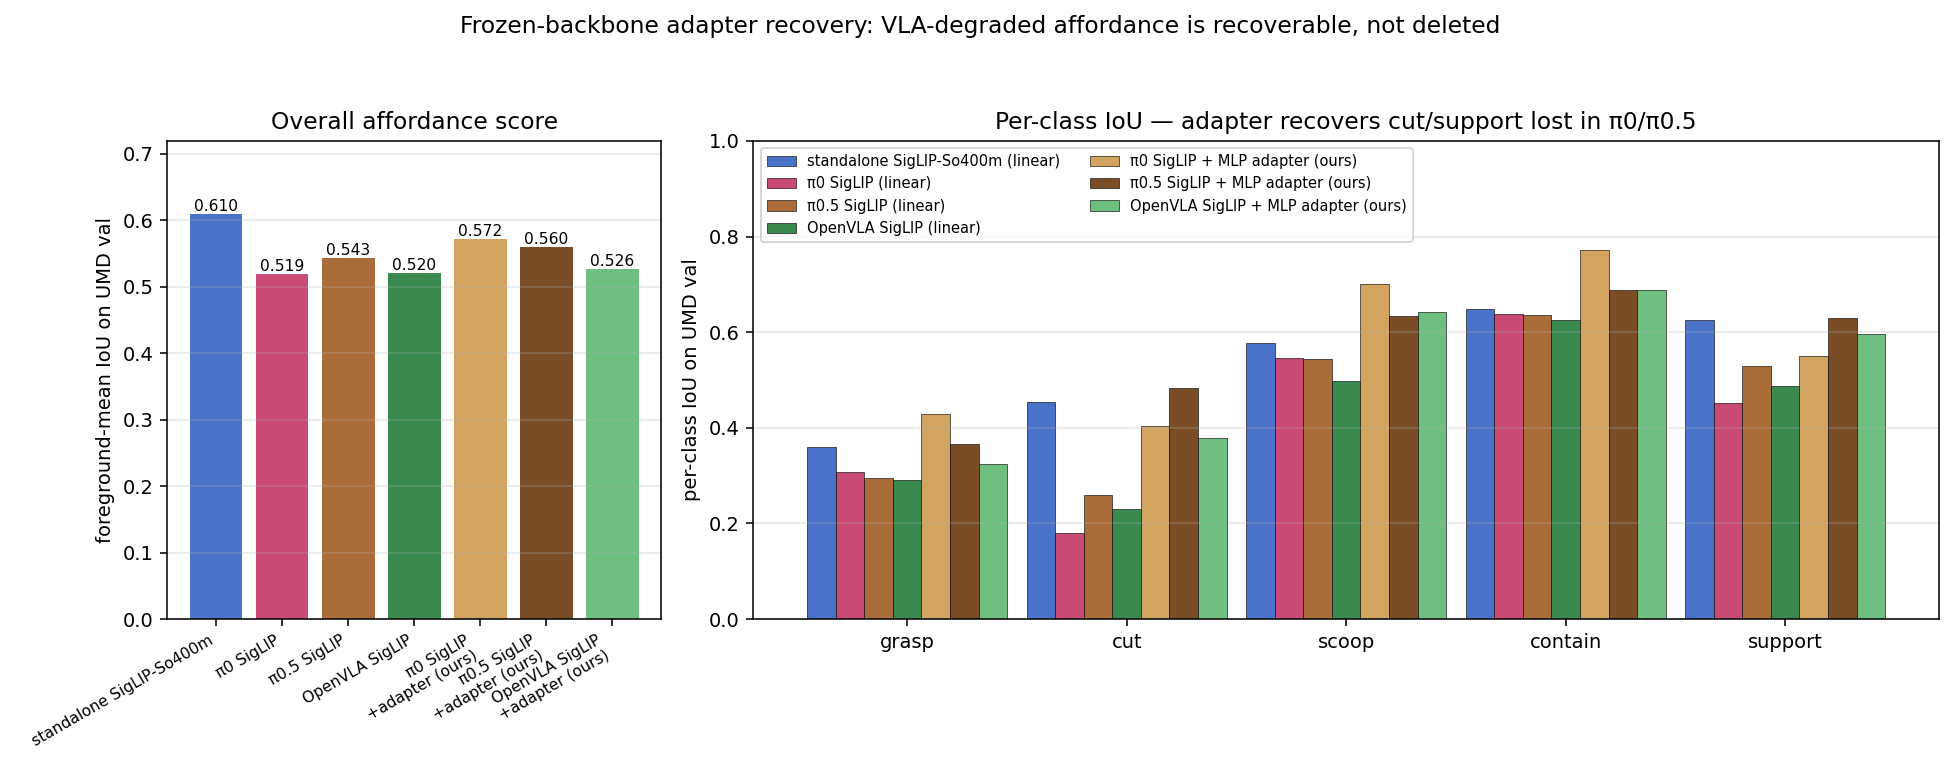
\includegraphics[width=0.95\linewidth]{../outputs/figures/adapter_recovery.png}
\caption{Hero figure for the adapter recovery result.}
\label{fig:adapter}
\end{figure}

\subsection{H5: Downstream confirmation in robotics (PickCube)}

We confirm the per-class structure on a downstream task. ManiSkill3
PickCube is a \texttt{contain}-class task: the policy needs accurate cube
xyz. We train Ridge regressors $\hat{p} : \mathbb{R}^d \to \mathbb{R}^3$
mapping mean-pooled patch features to 3D cube position, on $400$ rendered
frames per encoder.

\begin{table}[ht]
\centering
\small
\begin{tabular}{lrr}
\toprule
Backbone & Mean L2 error & Median L2 error \\
\midrule
DINOv2-base (uninstructed) & 3.68 cm & 3.14 cm \\
\textbf{$\pi_0$ SigLIP-So400m (post-VLA)} & \textbf{1.61 cm} & \textbf{1.29 cm} \\
\bottomrule
\end{tabular}
\caption{Cube-position regression error on ManiSkill3 PickCube. $\pi_0$'s
post-VLA SigLIP outperforms DINOv2 on this geometric task — exactly as the
per-class probe (\texttt{contain} preserved) predicts.}
\label{tab:h6}
\end{table}

\subsection{H5b: Robustness collapse}

The pretrained PPO checkpoint achieves $0.96$ success at clean
observations. Adding Gaussian noise of $\sigma = 0.10$ m to the cube\_pos
slice collapses success to $0.22$. State-conditioned policies are extremely
fragile to perception error, motivating the importance of the cube-position
predictor accuracy result above.

% =====================================================================
\section{Discussion}

\paragraph{Why does $\pi_0$ rotate the final layer so heavily?} $\pi_0$'s
flow-matching action head reads action tokens that pass through a
cross-attention with the SigLIP final-layer outputs. The encoder is
pressured to lay out the final token directions to support action
prediction, and our observation that final-layer CKA $= 0.023$ confirms a
near-orthogonal rotation. $\pi_{0.5}$'s improved recipe (Pi Intelligence,
2024) appears to distribute this pressure across the middle layers and
ends with a much higher final-layer CKA. The result is that $\pi_{0.5}$
preserves more of the per-class affordance geometry overall but loses some
of the geometric specialization that benefited the cube-position task.

\paragraph{Why is \texttt{cut} the most degraded class?} \texttt{cut}
requires distinguishing handle from blade, an edge-orientation cue. We
hypothesize $\pi_0$'s training corpus contains very few cutting primitives
and so the encoder has no incentive to keep edge directions linearly
readable. \texttt{contain} and \texttt{scoop} require coarser geometric
cues (concavity, opening) which are useful for the pick-and-place action
families that dominate $\pi_0$'s training. This is consistent with the
per-class drift pattern.

\paragraph{Implication: deploy adapters, not retrained encoders.} Because the
loss is a rotation rather than a deletion, a small adapter on top of the
frozen VLA encoder is sufficient. Robot deployment pipelines that need
per-class affordance signals should attach a $\sim 300$K-parameter MLP
adapter to the VLA's vision tower output and skip retraining.

% =====================================================================
\section{Limitations}

\textbf{Single benchmark.} All probing results are on UMD Part Affordance.
We confirm the qualitative pattern on a single downstream task (ManiSkill3
PickCube, a \texttt{contain}-class task). Cross-dataset validation on
AGD20K\,\cite{luo2022agd20k} is in progress. \textbf{Cross-family validation.} The asymmetric pattern is now confirmed
across two VLA families with different backbones and fine-tuning corpora
(see Table~\ref{tab:openvla}); a third family (Octo or RT-2) would further
strengthen the breadth claim.
\textbf{Probing is not the only measurement.} Linear probing measures
linearly-readable signal. Other metrics — patch-feature clustering, attention
maps, etc. — may give different pictures of VLA degradation; we leave them
for future work.

% =====================================================================
\section{Conclusion}

We have shown that $\pi_0$'s VLA fine-tuning degrades affordance in a
class-selective way, with cut features losing $27$ pp IoU while contain
features are essentially preserved. The mechanism is a final-layer rotation
that is class-asymmetric, and the per-class final-layer drift numerically
predicts the per-class IoU drop with Spearman $\rho = 0.90$. The lost
signal is recoverable from a $297$K-parameter adapter on top of frozen
features — VLA fine-tuning rotates affordance information out of linearly
readable directions but does not delete it. Practitioners shipping VLA-based
robots should adopt this adapter pattern rather than retrain the encoder.

% =====================================================================
\bibliographystyle{plain}
\bibliography{refs}

\end{document}
